\chapter{Introducción}

\section{Un poco de historia}

Desde que se lanzó en el año 2008 de la mano de la empresa taiwanesa HTC, el sistema operativo \textbf{Android}, desarrollado por Android Inc. y más tarde adquirido por Google,  ha extendido su uso alrededor de todo el mundo y actualmente cuenta con no menos de 3000 millones de dispositivos que dependen directamente de él, superando con creces su principal competidor iOS, de Apple.

Basado en el núcleo de Linux, el código fuente de Android es \textit{Open Source} (conocido como \textit{Android Open Source Project} o \textit{AOSP}) y está licenciado bajo la Licencia Apache.

En 2005, Google compró Android Inc. y dos años más tarde, en 2007, se creó la \textit{Open Handset Alliance}, un conjunto de fabricantes y desarrolladores de hardware, software y operadores de servicio que, junto a Google, lanzaron al mercado la primera versión del sistema operativo (Android 1.0: Apple Pie). No obstante, no fue hasta 2008 cuando apareció el primer teléfono inteligente, el HTC Dream, que utilizaba este sistema operativo.

Desde ese momento, el sistema operativo fue creciendo y desarrollándose cada vez más hasta alcanzar la versión actual, Android 11.

\section{Descripción del problema}

Los dispositivos tecnológicos portables, en concreto los teléfonos inteligentes, se han convertido en un pilar fundamental de nuestra vida. A través de estos dispositivos somos capaces de buscar información, mantener el contacto con gente de alrededor de todo el mundo a través de llamadas de teléfono o mensajería instantánea e incluso hacer compras por Internet. Esto ha supuesto un gran avance en materia de comunicaciones y desarrollo de software, pero también ha potenciado el desarrollo de software malicioso, maligno o malware que pone en peligro la seguridad de nuestros datos personales como la localización, los datos bancarios o la información de contacto. La seguridad de estos dispositivos se ha convertido en una preocupación creciente debido a la enorme cantidad de información almacenada en ellos, que en ocasiones ponen en riesgo no solo los datos personales del usuario del teléfono, sino también los de otras personas\hypersetup{citecolor=red}\cite{mobilesec}.

\subsection{Tipos de malware y dispositivos infectados}

Como bien sabemos, los teléfonos móviles son un punto de acceso a gran cantidad de nuestros datos personales, y, al igual que cualquier otro dispositivo, son vulnerables a los ataques cibernéticos que comprometen la privacidad y seguridad de dichos datos. Es inevitable que los dispositivos presenten alguna vulnerabilidad que los atacantes puedan usar, por pequeña que sea. No obstante, en la medida de lo posible, es conveniente mantener el dispositivo actualizado y controlado para minimizar los riesgos presentes y dificultar la entrada a atacantes a nuestro sistema. También es importante instalar aplicaciones de fuentes seguras que no supongan un peligro añadido.

Muchas veces las aplicaciones maliciosas se camuflan entre las aplicaciones benignas y pasan los controles de seguridad de \textit{Play Protect}, pues a simple vista parecen inofensivas. Difundir malware es muy sencillo: solo hay que ocultar con funcionalidades falsas la verdadera naturaleza de la aplicación. Eso ha hecho que las aplicaciones malware se extiendan casi sin control, en muchos casos, sin que los usuarios sean conscientes de que su dispositivo está infectado.

Hay distintos tipos de malware según el tipo de acción que llevan a cabo\hypersetup{citecolor=red}\cite{malwaredetection}:

\begin{itemize}
	\item \textbf{Virus}: necesitan de otro programa para poder propagarse. Están programados para ejecutarse una vez que hay una interacción del usuario (comúnmente llamado disparo o \textit{trigger}); contienen un fragmento de código maligno (\textit{payload}) que se copia en otros programas con diferentes efectos: borrado de archivos, bloqueo de acceso a ciertos archivos por cambios en los permisos o en la propiedad de directorios o archivos...
	\item \textbf{Gusanos}: están programados para reproducirse por sí mismos y difundirse a todos los dispositivos que sea posible. Normalmente se transmiten a través de SMS o MMS y no necesitan interacción del usuario para que se ejecuten.
	\item \textbf{Troyanos}: necesitan interacción del usuario en el dispositivo para poder ejecutarse. Se muestran como aplicaciones inofensivas, pero en realidad son programas engañosos que se instalan en nuestro sistema con una misión muy diferente a la que nosotros creemos.
	\item \textbf{Spyware}: recogen la información personal contenida en el dispositivo y la envían a servidores remotos sin el conocimiento ni consentimiento del usuario.
	\item \textbf{Ransomware}: son programas que cifran el dispositivo o los datos contenidos en él para solicitar después un rescate (del inglés, \textit{ransom}, que significa ``rescate''). El pago requerido alcanza cifras muy altas y se suele solicitar en forma de criptomonedas ya que son imposibles de rastrear.
\end{itemize}

Desde que se lanzó en el año 2008 hasta la actualidad, los ataques a teléfonos con sistema operativo Android han aumentado progresivamente con los años, creándose malware cada vez más sofisticado y complejo que pasa desapercibido al ser difícil de detectar. En la Figura~\ref{fig:avtest} se puede ver el aumento de nuevas variantes de malware entre los años 2010 y principios de 2019.

\begin{figure}[H]
\centering
	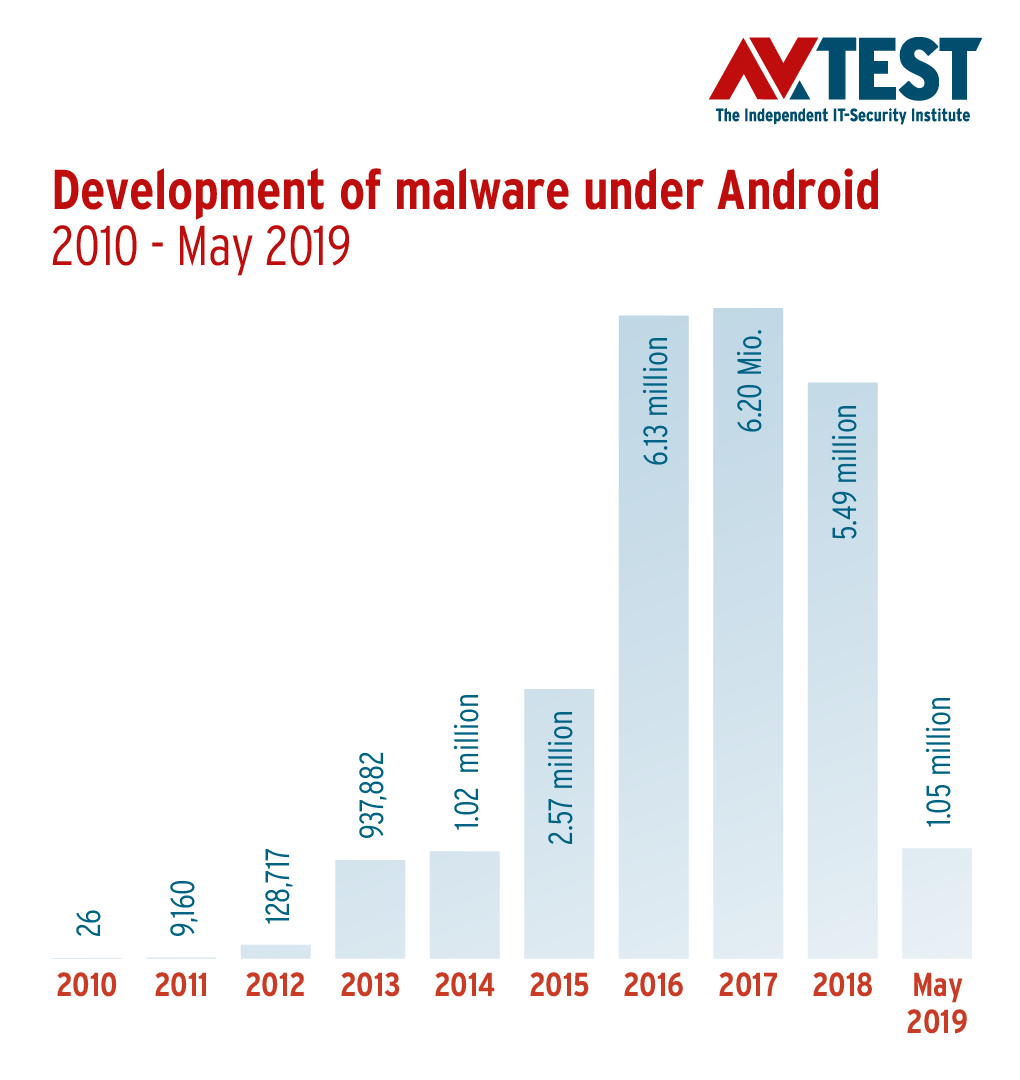
\includegraphics[scale=0.25]{img/2010-mayo2019.png}
	\caption{Nuevo malware desarrollado \textit{(AV-TEST, 2019-2020)}}
	\label{fig:avtest}
\end{figure}

El número de dispositivos infectados durante los dos últimos años supone una cifra preocupante (ver Figura~\ref{fig:infectados}).

\begin{figure}[H]
\centering
	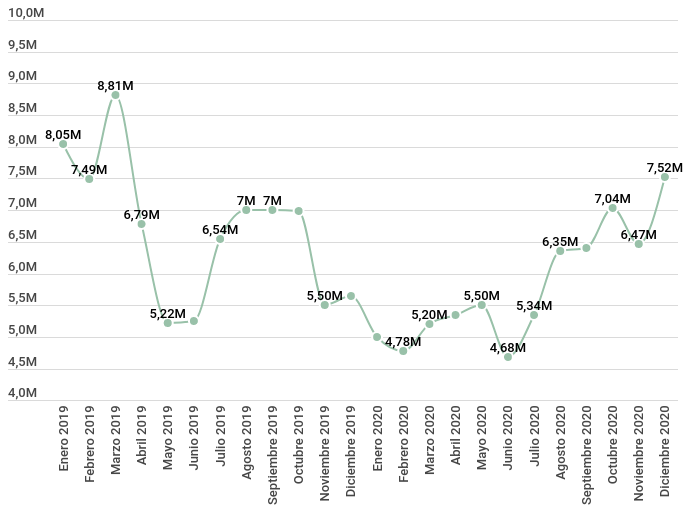
\includegraphics[scale=0.35]{img/2019-2020.png}
	\caption{Dispositivos infectados entre 2019 y 2020 \textit{(Kaspersky, 2020)}}
	\label{fig:infectados}
\end{figure}

El malware presente en los dispositivos Android siempre se ha mantenido en una cifra que supera el millón de dispositivos infectados; a pesar de tener altibajos sigue siendo una cifra demasiado alta. La naturaleza de este trabajo es colaborar con el descenso de dichas cifras.

\subsection{Seguridad en Android}

Android es un sistema con una arquitectura por capas que aisla unas partes del dispositivo de otras y facilita la abstracción en cuanto a programación de aplicaciones. Esto dificulta los ataques en gran medida, pero a pesar de ser robusto, el sistema operativo puede contener agujeros de seguridad que los atacantes pueden utilizar. Su frecuencia de actualización recomendada es mensual, publicandose parches de seguridad de manera continuada para cubrir las vulnerabilidades encontradas y mantener el dispositivo, y por tanto los datos, a salvo.

A pesar de ello, los atacantes aprovechan los puntos débiles y las vulnerabilidades del día cero (\textit{zero-day vulnerabilities}) para acceder a los dispositivos de una forma u otra y extraer información, por lo general con objetivos económicos.

En muchos casos el problema de seguridad radica en el uso que hace el usuario del dispositivo en lugar de problemas en el propio sistema. La seguridad de los teléfonos Android depende tanto del sistema, como de aplicaciones y del usuario. Vamos a ver ahora las diferentes capas que forman la seguridad en Android\hypersetup{citecolor=red}\cite{seclayers}.

\subsubsection{Seguridad a nivel de SO}

El sistema operativo de Android utiliza tres características propias del núcleo de Linux para proteger el dispositivo:

\begin{itemize}
	\item \textit{\textbf{Sandboxing}}: supone aislar los procesos unos de otros y del propio SO para así evitar que aplicaciones maliciosas interactúen con otras apps y limitar el acceso al sistema operativo. También el proceso de comunicación entre aplicaciones es aislado mediante el uso del \textit{User ID} o \textit{UID}, que permite gestionar el acceso a aplicaciones de manera individual en lugar de poder acceder al sistema completo.
	\item \textit{\textbf{Rooting}}: Android mantiene la cuenta del usuario y la del \textit{root} como cuentas separadas. El usuario no tiene acceso a ciertas operaciones o archivos potencialmente sensibles. Esto previene que, si una aplicación maliciosa entra en el sistema e intenta engañar al usuario para que le de acceso a los mismos permisos que posee el \textit{root}, el usuario no pueda concederlos. No obstante, y aunque no es una práctica recomendada, para superar las limitaciones del aislamiento de procesos Android permite que el usuario ``rootee'' el sistema, es decir, que adquiera permisos de \textit{root} para tener acceso a todos los archivos y operaciones que se pueden llevar a cabo.
	\item \textit{\textbf{Verified boot}}: también llamado arranque verificado, es un proceso que asegura que el sistema operativo que se arranca en el dispositivo es el original y no una copia que puede ser maliciosa. El arranque verificado lleva a cabo una serie de verificaciones en cadena (similar a la forma en que se llevan a cabo las verificaciones en la tecnología \textit{blockchain}), desde el hardware hasta las particiones de memoria. En el caso de que haya algo alterado en la cadena, se invalida la verificación y se alerta al usuario del comportamiento extraño.
\end{itemize}

Este es el primer nivel de protección y que, en gran medida, no depende del usuario (a menos que se ``rootee'' el teléfono).

\subsubsection{Seguridad a nivel de aplicación}

Gracias a la abstracción proporcionada por las capas que forman la arquitectura de Android, este nivel supone que el nivel de seguridad del SO funciona correctamente. Al igual que el nivel anterior, está dividido en varias partes que se entrelazan.

\begin{itemize}
	\item \textbf{Almacenamiento}: puesto que los datos almacenados es el objetivo principal por el que un atacante lleva a cabo un ataque, Android asegura los datos guardados según la sensibilidad de éstos.
	\begin{itemize}
		\item Los datos de una aplicación que están guardados en el almacenamiento interno solo pueden ser vistos por dicha aplicación. Esto significa que las aplicaciones no pueden ver los archivos guardados en los directorios que pertenecen a otras aplicaciones.
		\item Los datos guardados en el almacenamiento externo pueden ser leídos y modificados por cualquier aplicación, lo que significa que la información contenida puede ser alterada por una aplicación que un atacante haya introducido en el sistema. No obstante, a partir de Android 11, se ha introducido el ``almacenamiento de ámbito'' (\href{https://developer.android.com/about/versions/11/privacy/storage}{\textcolor{blue}{\textit{scoped storage}}}\footnote[1]{https://developer.android.com/about/versions/11/privacy/storage}), con el que la mayor parte de los riesgos asociados con el almacenamiento externo han sido eliminados.
		\item La compartición de información entre aplicaciones se lleva a cabo a través de los \textit{content providers}, que permiten abstraer a las aplicaciones del almacenamiento. Añaden una capa de seguridad, pues los \textit{content providers} requieren permisos de lectura y escritura para poder acceder a los datos.
	\end{itemize}
	\item \textit{\textbf{Interprocess communication, IPC}}: Android mantiene la comunicación entre procesos segura, utilizando tres mecanismos: \textit{binder} y \textit{messenger} (utilizados para implementar llamadas remotas a procemientos) que proporcionan una interfaz para que las llamadas entre aplicaciones y servicios del sistema sean seguras; y los \textit{intents}, que son el mecanismo a través del que se transmiten los datos.
	\item \textbf{Firma de aplicaciones}: Google obliga a que las aplicaciones estén firmadas por los desarrolladores para que puedan ser publicadas en \textit{Google Play}. Las aplicaciones provenientes de fuentes desconocidas también deben estar firmadas, ya que de lo contrario Android no permite su instalación. Esto se debe a que la firma es el primer paso durante el aislamiento de apliaciones anteriormente explicado (\textit{sandboxing}), y sin firma, el sistema operativo no permite crear el entorno aislado.
	\item \textbf{Permisos a nivel de aplicación}: esta medida se tratará con más detalle en el siguiente apartado ya que \textit{Android Shield} versa sobre ella.
\end{itemize}

\subsection{Permisos para asegurar el dispositivo}
\label{sec121}

En Android, destaca el amplio conjunto de permisos que controla el acceso a partes especificas del sistema y a funcionalidades que cada aplicación puede llevar a cabo. El acceso a las distintas partes del dispositivo (a partes hardware como el micrófono, la cámara o los altavoces), las acciones que se pueden realizar sobre los datos (guardado, editado, borrado...) o la recogida y eliminación de información (tanto de archivos individuales, como de directorios completos así como de la memoria interna y externa) están estrictamente controladas por este sistema de permisos.

Si nos fijamos en la Figura~\ref{fig:layers}, en la esquina inferior derecha se situaría el acceso sin restricciones a todas los componentes del sistema, el uso de cada componente con la mayor libertad posible. Eso significa que los permisos son la última barrera de defensa del sistema Android para detener al malware de acceder a todo.

\begin{figure}[H]
\centering
	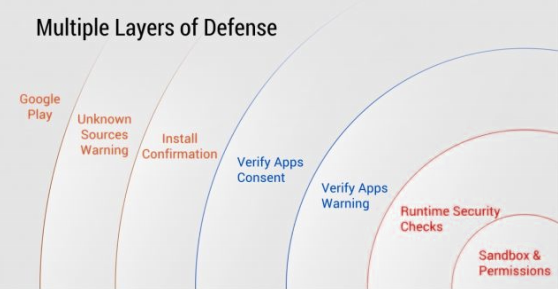
\includegraphics[scale=0.65]{img/layers.png}
	\caption{Capas de seguridad en Android \textit{(Rahimi, 2019)}}
	\label{fig:layers}
\end{figure}

Los permisos constituyen la última medida de seguridad antes de que el dispositivo se convierta en uno vulnerable que no restringe el acceso a las partes más delicadas. Eso significa que si el usuario no presta atención y otorga permisos sin ton ni son, la última defensa del dispositivo habrá caído y será vulnerable, pues no habrá nada que frene el acceso libre a la información contenida en él. Es aquí donde radica el verdadero problema: una vez que el malware ha conseguido acceso, la información queda a mercer del atacante y desde ese momento puede hacer lo que desee con ella.

Algunos permisos son otorgados directamente al instalar la aplicación, mientras que otros deben ser otorgados por el usuario durante la ejecución de la aplicación. Los permisos se declaran en el archivo \textit{AndroidManifest.xml} y su gestión ha variado con la versión de la API de Android (véase\hypersetup{citecolor=red}\cite{history} y\hypersetup{citecolor=red}\cite{sharma} para ver otras caracterísicas añadidas en cada versión). 

\begin{itemize}
	\item Desde \textbf{Android 1.0} (API 1) hasta \textbf{Android 2.3.3} (API 10) la seguridad del sistema operativo es muy básica y no hay permisos definidos.
	\item En \textbf{Android 3.0} (API 11) se introducen por primera vez los permisos a nivel de aplicación, específicos para poder acceder al almacenamiento interno.
	\item En \textbf{Android 4.3} (API 18) se introduce la gestión de permisos a nivel de aplicación mediante un sistema de control denominado \textit{App Ops}, una característica oculta por defecto. En la siguiente actualización del sistema, esta característica se elimina.
	\item En \textbf{Android 6.0} (API 23) se incluye la gestión de permisos en tiempo de ejecución, aquellos que se otorgan cuando la aplicación se ejecuta. Además, ahora los permisos se conceden de manera individual; al instalar la aplicación no se tienen que conceder todos o ninguno, pueden concederse solo algunos (similar al sistema \textit{App Ops}). Hasta esta versión si no se concedían todos los permisos solicitados a una aplicación, ésta no podía funcionar.
	\item En \textbf{Android 8.0} (API 26), y la subsecuente actualización, \textbf{Android 8.1} (API 27), fueron las primeras versiones en introducir el sistema de \textit{Play Protect} y mejorar el sistema de permisos.
	\item En la versión \textbf{Android 10.0} (API 29) se restringe el permiso de las aplicaciones para acceder a los datos de localización si están en \textit{background} (a menos que el usuario permita específicamente que la aplicación recoja dichos datos cuando no está ejecutándose en primer plano).
	\item En la última versión de Android, la 11.0 (API 30), se introducen los permisos \textit{one time} para el acceso a cámara, micrófono y localización. Los permisos \textit{one time} son aquellos que el usuario aprueba o deniega en el momento de utilizar la aplicación.
\end{itemize}

Google califica los permisos que el usuario gestiona (los únicos sobre los que tiene poder, pues es el usuario quien concede a la aplicación el acceso o, por el contrario, lo revoca) como permisos peligrosos (\textit{dangerous permissions}) porque acceden a partes del dispositivo o hacen uso de ciertas funcionalidades o información que pueden ser sensibles y poner en riesgo la privacidad del usuario. Mediante el control riguroso de estos permisos peligrosos, el sistema de seguridad de Android se ve reforzado y es eficaz para detener posibles amenazas.

Los usuarios que acostumbran a tratar con la tecnología, en particular a tratar con Android, suelen ser conscientes de los peligros que existen si se despreocupan las diferentes capas de seguridad, especialmente la última, pues es aquella en la que un usuario común tiene más control. Otorgar y revocar permisos a las aplicaciones está al alcance de todos, pero hacerlo sin un mínimo conocimiento de causa puede acarrear problemas. Pero a pesar de esto, todos los usuarios, estén o no acostumbrados a la tecnología y a la gestión de permisos, pueden caer en el error de dejar entrar malware a su sistema, por lo general por ignorancia o desconocimiento.

Como se explica en \hypersetup{citecolor=red}\cite{porter} y en\hypersetup{citecolor=red}\cite{khantoon}, Android supone que el usuario sabe de antemano lo que conlleva la activación de cada permiso y, por tanto, será capaz de determinar cuándo un permiso no necesita ser activado o cuando debe ser desactivado para minimizar riesgos. No obstante, la realidad dista mucho de esta suposición: muchas veces los usuarios se olvidan que han concedido un permiso determinado a una aplicación o incluso ignoran el problema, ya que desconocen los peligros que acarrea mantener el permiso activo. El sistema de permisos puede ayudar mucho a un usuario a controlar que no sufra ataques que amenacen su privacidad, pero para ello hay que tener unas nociones previas que la mayoría no tienen. Es aquí donde los atacantes pueden sacar provecho de las vulnerabilidades del sistema. Como se explica en \hypersetup{citecolor=red}\cite{bassole}, los atacantes se aprovechan de las vulnerabilidades causadas por la solicitud de permisos y crean aplicaciones maliciosas en las que declaran muchos permisos\hypersetup{citecolor=red}\cite{attandck} que después difunden camufladas como aplicaciones benignas. Si un usuario descarga una aplicación de una fuente no segura y concede ciertos permisos sin detenerse a pensar qué uso hará la aplicación con la información contenida en su sistema, los atacantes podrán acceder a todas aquellas partes del dispositivo que deseen, extraer toda la información que quieran, hacer llamadas de teléfono, enviar mensajes SMS o recolectar información sobre los contactos del usuario.

\section{Consecuencias de la falta de seguridad}

\subsection{Peligros del malware en usuarios}

Es obvio que tener malware instalado en nuestro dispositivo conlleva riesgos, pero nunca somos conscientes de hasta qué punto es peligroso. Estamos expuestos sin estar al tanto de ello.

El mayor peligro al que un usuario común puede enfrentarse es el secuestro de datos o el robo de información (credenciales de acceso a diferentes cuentas, tanto en cuentas bancarias, como redes sociales como cualquier otro acceso posible). Aunque en principio atacar a un usuario común podría sonar poco llamativo o una pérdida de tiempo, los atacantes saben como utilizar la información de la que disponen para extorsionar a las víctimas y lucrarse\hypersetup{citecolor=red}\cite{risks}.

\subsection{Peligros del malware en empresas y negocios}

En cuanto a los ataques a las compañías, suceden a diario. No obstante, muchos de estos ataques son detenidos a tiempo y no se sufren daños mayores.

Un ataque exitoso puede causar graves perjuicios, hasta el punto de incluso acabar con la empresa. Los daños ocasionados varían y pueden alcanzar costes millonarios además de la pérdida de clientes, filtración de datos, (tanto los datos personales de los clientes como los datos de la propia compañía), secuestro de información mediante sofisticados ransomware o recolección de información para después venderla a los competidores\hypersetup{citecolor=red}\cite{risks}.

Se estima que cada año la pérdida monetaria mundial derivada del cibercrímen asciende a la cifra estimada de entre 600 billones y un trillón de dólares americanos\hypersetup{citecolor=red}\cite{mcafee}. Cualquier compañía, grande o pequeña es víctima de un ataque si es conveniente, aunque los atacantes se centran en las empresas pequeñas pues las consideran los eslabones débiles: una empresa pequeña con poca ganancia anual tiende a ceder en la seguridad de sus sistemas, dejándolos vulnerables y en muchas ocasiones sin ningún tipo de monitorización, lo que los convierte en un blanco fácil de atacar.

Recientemente, durante el año 2019, la empresa multimillonaria \textit{Facebook} sufrió la filtración de los datos de 530 millones de usuarios, entre los que se encontraban los números de teléfono, nombres completos, direcciones y correos electrónicos\hypersetup{citecolor=red}\cite{fb}.

Ninguna empresa ni ningún usuario está a salvo de un ataque, por eso la seguridad de los dispositivos debería ser una de las mayores prioridades.

\section{Objetivo de este proyecto}

La idea principal de este proyecto es crear una aplicación que ayude a mejorar la seguridad del dispositivo Android haciendo una clasificación de las aplicaciones instaladas en aplicaciones benignas o maliciosas.

Para ello, mediante los permisos declarados en el \textit{AndroidManifest.xml}, y usando varias técnicas de \textit{Machine Learning} combinadas de manera secuencial, se ha entrenado un modelo con distintos \textit{datasets} para que clasifique dichas aplicaciones y muestre la estimación hecha para cada una, de manera que el usuario sepa si su sistema ha sido infectado por algún malware camuflado en forma de aplicación.

Esta aplicación tiene como objetivo ayudar a un usuario común a saber si una aplicación instalada es maliciosa sin que se vea obligado a entender el entramado y los riesgos de seguridad que supone tener activos algunos permisos.